% !TEX program = xelatex
\documentclass[10pt,letterpaper,twocolumn]{article}

% === GEOMETRY ===
\usepackage[top=0.75in, bottom=0.75in, left=0.75in, right=0.75in]{geometry}

% === FONTS ===
\usepackage{fontspec}
\usepackage{unicode-math}

\setmainfont{Latin Modern Roman}
\setsansfont{Latin Modern Sans}

% Custom AC fonts
\newfontfamily\acbold{ywft-processing-bold}[
  Path=../../system/public/type/webfonts/,
  Extension=.ttf
]
\newfontfamily\aclight{ywft-processing-light}[
  Path=../../system/public/type/webfonts/,
  Extension=.ttf
]
\newfontfamily\kidlispfont{ComicRelief-Regular}[
  Path=fonts/,
  Extension=.ttf
]
\newfontfamily\kidlispbold{ComicRelief-Bold}[
  Path=fonts/,
  Extension=.ttf
]
\setmonofont{Latin Modern Mono}[Scale=0.85]

% === PACKAGES ===
\usepackage{xcolor}
\usepackage{titlesec}
\usepackage{enumitem}
\usepackage{booktabs}
\usepackage{tabularx}
\usepackage{multicol}
\usepackage{fancyhdr}
\usepackage{hyperref}
\usepackage{graphicx}
\graphicspath{{figures/}}
\usepackage{ragged2e}
\usepackage{microtype}
\usepackage{listings}
\usepackage{natbib}
\usepackage[colorspec=0.92]{draftwatermark}

% === COLORS (AC palette) ===
\definecolor{acpink}{RGB}{180,72,135}
\definecolor{acpurple}{RGB}{120,80,180}
\definecolor{acdark}{RGB}{64,56,74}
\definecolor{acgray}{RGB}{119,119,119}
\definecolor{klbrand}{RGB}{205,92,155}
\definecolor{klcyan}{RGB}{112,214,255}
\definecolor{kldark}{RGB}{48,43,58}
\definecolor{draftcolor}{RGB}{205,92,155}

% === DRAFT WATERMARK ===
\DraftwatermarkOptions{
  text=WORKING DRAFT,
  fontsize=3cm,
  color=draftcolor!18,
  angle=45,
  pos={0.5\paperwidth, 0.5\paperheight}
}

% === KIDLISP SYNTAX COLORS ===
\definecolor{klfn}{RGB}{0,136,170}
\definecolor{klform}{RGB}{119,51,170}
\definecolor{klrepeat}{RGB}{170,0,170}
\definecolor{klnum}{RGB}{204,0,102}
\definecolor{klstr}{RGB}{170,120,0}
\definecolor{klcmt}{RGB}{102,102,102}
\definecolor{klmath}{RGB}{0,136,0}
\definecolor{klvar}{RGB}{204,102,0}
\definecolor{klembed}{RGB}{0,136,0}

% KidLisp inline color macros
\newcommand{\kn}[1]{\textcolor{klnum}{#1}}
\newcommand{\kt}[1]{\textcolor{klstr}{#1}}
\newcommand{\kv}[1]{\textcolor{klvar}{#1}}
\newcommand{\ke}[1]{\textcolor{klembed}{\textbf{#1}}}
\newcommand{\km}[1]{\textcolor{klmath}{#1}}

% === HYPERREF ===
\hypersetup{
  colorlinks=true,
  linkcolor=acpurple,
  urlcolor=acpurple,
  citecolor=acpurple,
  pdfauthor={Jeffrey Alan Scudder},
  pdftitle={KidLisp '26: Un Lisp mínimo para arte generativo},
}

% === SECTION FORMATTING ===
\titleformat{\section}
  {\normalfont\bfseries\normalsize\uppercase}
  {\thesection.}
  {0.5em}
  {}
\titlespacing{\section}{0pt}{1.2em}{0.3em}

\titleformat{\subsection}
  {\normalfont\bfseries\small}
  {\thesubsection}
  {0.5em}
  {}
\titlespacing{\subsection}{0pt}{0.8em}{0.2em}

% === HEADER/FOOTER ===
\pagestyle{fancy}
\fancyhf{}
\renewcommand{\headrulewidth}{0pt}
\fancyhead[C]{\footnotesize\color{acpink}\textit{Borrador de trabajo --- no citar}}
\fancyfoot[C]{\footnotesize\thepage}

% === CUSTOM COMMANDS ===
\newcommand{\acdot}{{\color{acpink}.}}
\newcommand{\kidlisp}{\textsc{KidLisp}}

% === LISTINGS ===
\lstdefinelanguage{kidlisp}{
  morekeywords=[1]{wipe,ink,line,box,circle,tri,plot,flood,shape,zoom,scroll,spin,blur,contrast,embed,layer,width,height,frame,time,wiggle,melody,mic,suck,sort,form,trans,cube,move,scale,hop,overtone,resolution,write,text,type,stamp,paste,point,poly,noise,fade,pan,unpan,mask,unmask,flip},
  morekeywords=[2]{def,let,if,cond,once,later,lambda,do},
  morekeywords=[3]{repeat},
  morekeywords=[4]{random,sin,cos,tan,floor,ceil,round,abs,sqrt,min,max},
  sensitive=true,
  morecomment=[l]{;},
  morestring=[b]",
  escapeinside={|}{|},
}
\lstset{
  language=kidlisp,
  basicstyle=\ttfamily\small,
  keywordstyle=[1]\color{klfn}\bfseries,
  keywordstyle=[2]\color{klform}\bfseries,
  keywordstyle=[3]\color{klrepeat}\bfseries,
  keywordstyle=[4]\color{klmath},
  commentstyle=\color{klcmt}\itshape,
  stringstyle=\color{klstr},
  breaklines=true,
  frame=single,
  rulecolor=\color{acgray!30},
  backgroundcolor=\color{acgray!5},
  xleftmargin=0.5em,
  xrightmargin=0.5em,
  aboveskip=0.5em,
  belowskip=0.5em,
}

\lstdefinelanguage{json}{
  basicstyle=\ttfamily\small,
  stringstyle=\color{acpink},
  morestring=[b]",
  literate=
    {:}{{{\color{acgray}:}}}{1}
    {,}{{{\color{acgray},}}}{1}
    {\{}{{{\color{acgray}\{}}}{1}
    {\}}{{{\color{acgray}\}}}}{1},
}

% === LIST SETTINGS ===
\setlist[itemize]{nosep, leftmargin=1.2em, itemsep=0.1em}
\setlist[enumerate]{nosep, leftmargin=1.2em}

% === COLUMN SEPARATION ===
\setlength{\columnsep}{1.8em}

% === PARAGRAPH SETTINGS ===
\setlength{\parindent}{1em}
\setlength{\parskip}{0.3em}

\begin{document}

% ============ TITLE BLOCK ============

\twocolumn[{%
\begin{center}

\includegraphics[height=4em]{pals}\par\vspace{0.5em}
{\kidlispbold\fontsize{26pt}{30pt}\selectfont\color{kldark} Kid{\color{klbrand}Lisp} '26}\par
\vspace{0.2em}
{\kidlispfont\fontsize{11pt}{13pt}\selectfont\color{klbrand} Un Lisp mínimo para arte generativo}\par
\vspace{0.6em}
{\normalsize Jeffrey Alan Scudder}\par
{\small\color{acgray} Aesthetic Inc.}\par
{\small\color{acgray} ORCID: \href{https://orcid.org/0009-0007-4460-4913}{0009-0007-4460-4913}}\par
\vspace{0.3em}
{\small\color{acpurple} \url{https://kidlisp.com} \enspace$\cdot$\enspace \url{https://aesthetic.computer}}\par
\vspace{0.6em}
\rule{\textwidth}{1.5pt}
\vspace{0.5em}
\end{center}

\begin{center}
{\small\color{acpink}\textbf{[ borrador de trabajo --- no citar ]}}
\end{center}
\vspace{0.3em}

\begin{quote}
\small\noindent\textbf{Resumen.}
\kidlisp{} es un dialecto Lisp mínimo diseñado para arte generativo y experiencias audiovisuales interactivas. Se ejecuta dentro de Aesthetic Computer, una plataforma de computación creativa basada en navegador. Los programas se almacenan en MongoDB, se les asignan códigos alfanuméricos cortos y son ejecutables en una URL. Un evaluador de recorrido de árbol de 15.000 líneas proporciona 118 funciones integradas que abarcan dibujo, color, transformación, matemáticas, animación y audio---sin E/S de archivos, redes ni manipulación general de cadenas---lo que hace seguro ejecutar código arbitrario enviado por usuarios. Describimos el diseño del lenguaje, la infraestructura de almacenamiento y distribución, la cadena de procesamiento de medios, y reportamos sobre la adopción por parte de 59 autores que han creado más de 16.000 programas. Sostenemos que integrar la distribución social directamente en un lenguaje de dominio específico---en lugar de añadirla---produce prácticas de programación creativa cualitativamente diferentes.
\end{quote}
\vspace{0.5em}
}]

% ============ 1. INTRODUCCIÓN ============

\section{Introducción}

Los entornos de programación creativa típicamente requieren que los usuarios aprendan un lenguaje de programación de propósito general antes de producir salida visual o sonora. Processing~\citep{reas2007processing} usa Java; p5.js~\citep{mccarthy2015p5js} usa JavaScript; Sonic Pi~\citep{aaron2016sonic} usa constructos similares a Ruby. Aunque estas herramientas han reducido dramáticamente la barrera de acceso a la expresión computacional, aún demandan familiaridad con variables, funciones, flujo de control y---en muchos casos---un entorno de desarrollo local.

\kidlisp{} parte de una pregunta diferente: \emph{¿cuál es el lenguaje más pequeño que puede producir arte generativo interesante?} La respuesta es un Lisp con funciones integradas cuidadosamente elegidas, sin procedimientos definidos por el usuario, y un entorno de ejecución nativo del navegador que no requiere instalación. Un programa animado completo puede ser una sola línea:

\begin{lstlisting}
(ink |\kt{rainbow}|) (repeat |\kn{100}| |\kv{i}|
  (circle (wiggle width) (wiggle height) |\kn{10}|))
\end{lstlisting}

El diseño está motivado por observaciones de No Paint~(2020), una herramienta de pixel art cuya comunidad de usuarios no técnicos demostró que las personas aprenden computación a través de la participación social en software que aman. \kidlisp{} extiende esta idea a un lenguaje de programación: cada programa es inmediatamente compartible por un código corto, visible en una URL e incrustable dentro de otros programas.

Este artículo describe el diseño del lenguaje~(\S\ref{sec:design}), la arquitectura del evaluador~(\S\ref{sec:architecture}), la infraestructura de almacenamiento y distribución~(\S\ref{sec:infrastructure}), la cadena de procesamiento de medios~(\S\ref{sec:media}), y los datos de adopción~(\S\ref{sec:evaluation}).

\begin{figure}[t]
\centering
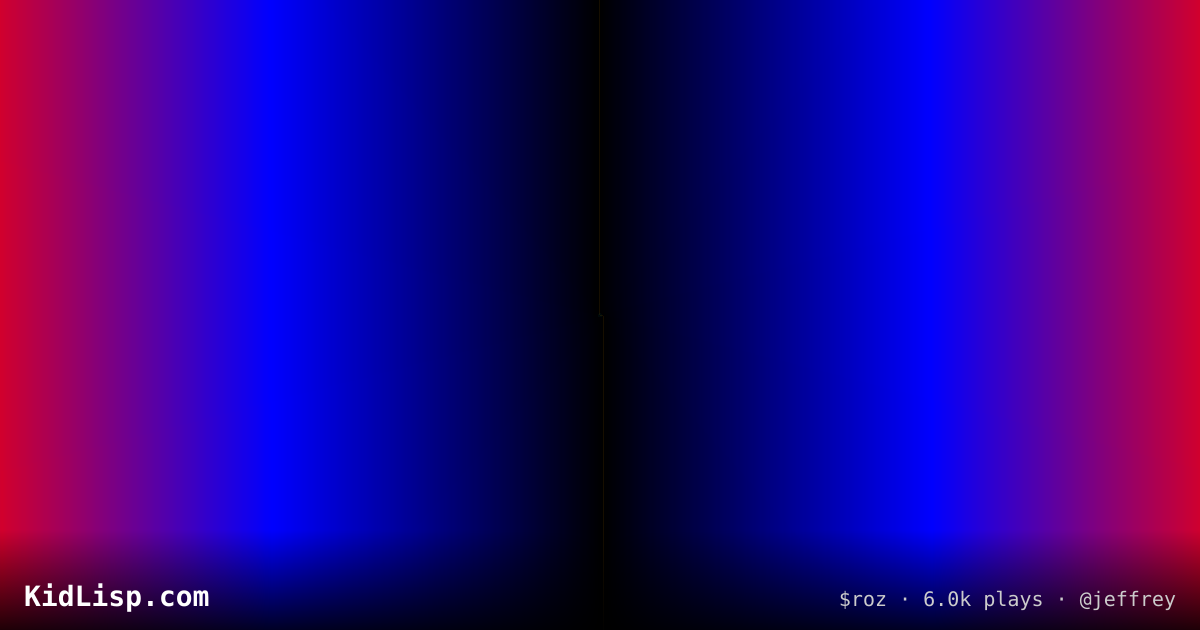
\includegraphics[width=\columnwidth]{kidlisp-og-mosaic.png}
\caption{Un programa \kidlisp{} destacado (\texttt{\$roz}) tal como lo renderiza el servicio oven para vistas previas sociales Open Graph. La superposición muestra el código del programa, el conteo de reproducciones y el identificador del autor.}
\label{fig:og}
\end{figure}

% ============ 2. DISEÑO DEL LENGUAJE ============

\section{Diseño del lenguaje}
\label{sec:design}

\kidlisp{} es un lenguaje de S-expresiones. Cada programa es una secuencia de expresiones evaluadas de arriba a abajo, produciendo efectos secundarios en un contexto HTML Canvas 2D, un contexto WebGL, un grafo Web Audio, o alguna combinación de estos.

\subsection{Principios de diseño}

\begin{enumerate}
  \item \textbf{Cada expresión dibuja.} Un \kidlisp{} válido produce salida visible. No hay \texttt{main}, no hay importaciones, no hay código repetitivo.
  \item \textbf{Plano sobre profundo.} Los programas se componen incrustando otros programas, no definiendo abstracciones. Esto mantiene el código legible de un vistazo.
  \item \textbf{Seguro por construcción.} Sin E/S de archivos, sin redes, sin mutación de estado externo. Los programas están aislados por la ausencia de primitivas peligrosas en el lenguaje.
  \item \textbf{Social por defecto.} Cada programa obtiene un código corto y una URL. Compartir es el mecanismo de distribución, no un añadido posterior.
\end{enumerate}

\subsection{Categorías de funciones}

Las 118 funciones integradas abarcan 12 categorías (Tabla~\ref{tab:functions}).

\begin{table}[h]
\small
\centering
\begin{tabularx}{\columnwidth}{lrX}
\toprule
\textbf{Categoría} & \textbf{n} & \textbf{Ejemplos} \\
\midrule
Gráficos & 9 & \texttt{wipe}, \texttt{ink}, \texttt{line}, \texttt{box}, \texttt{circle} \\
Transformaciones & 11 & \texttt{scroll}, \texttt{zoom}, \texttt{spin}, \texttt{blur}, \texttt{suck} \\
Matemáticas & 14 & \texttt{+}, \texttt{sin}, \texttt{cos}, \texttt{random}, \texttt{wiggle} \\
Colores & 19 & Nombres CSS + \texttt{rainbow}, \texttt{zebra} \\
Sistema & 9 & \texttt{width}, \texttt{height}, \texttt{frame}, \texttt{fps} \\
3D & 8 & \texttt{cube}, \texttt{form}, \texttt{trans}, \texttt{move} \\
Audio & 6 & \texttt{mic}, \texttt{melody}, \texttt{overtone} \\
Control & 7 & \texttt{def}, \texttt{if}, \texttt{repeat}, \texttt{once}, \texttt{later} \\
Texto & 4 & \texttt{write}, \texttt{type}, \texttt{paste} \\
Entrada & 3 & \texttt{pen}, \texttt{touch} \\
Composición & 4 & \texttt{embed}, \texttt{layer}, \texttt{fade} \\
Datos & 4 & \texttt{let}, \texttt{list}, \texttt{get}, \texttt{set} \\
\midrule
\textbf{Total} & \textbf{118} & \\
\bottomrule
\end{tabularx}
\caption{Funciones integradas por categoría.}
\label{tab:functions}
\end{table}

\begin{figure}[t]
\centering
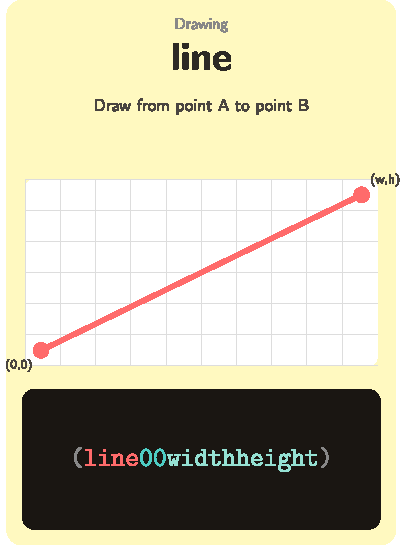
\includegraphics[height=4.5cm]{card-line.pdf}%
\hfill%
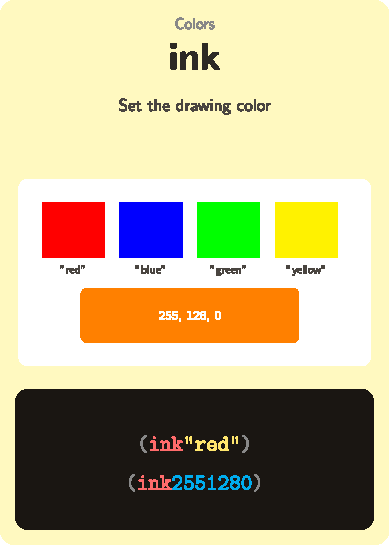
\includegraphics[height=4.5cm]{card-ink.pdf}
\caption{Tarjetas de referencia de \kidlisp{} para las funciones \texttt{line} e \texttt{ink}, mostrando la sintaxis y la salida de coordenadas. Las tarjetas se distribuyen como ilustraciones SVG en \texttt{kidlisp.com/cards}.}
\label{fig:cards}
\end{figure}

\subsection{Sintaxis temporal}

\kidlisp{} proporciona operadores temporales que programan la evaluación de expresiones sin bucles explícitos ni callbacks:

\begin{lstlisting}
|\kt{2.5s}| (wipe |\kt{red}|)           ; después de 2,5 segundos
|\kt{1s...}| (spin |\kn{5}|)            ; repetir cada segundo
|\kt{3s!}| (write "Done" |\kn{10}| |\kn{10}|)  ; ejecutar exactamente una vez a 3s
|\kt{30f}| (ink |\kt{blue}|)             ; después de 30 fotogramas
\end{lstlisting}

El sufijo \texttt{s} denota segundos, \texttt{f} denota fotogramas, \texttt{...} denota repetición, y \texttt{!} denota ejecución única. Estos operadores se componen: \texttt{0.5s... (ink (random 255) (random 255) (random 255))} produce un cambio de color cada medio segundo.

\subsection{Lo que KidLisp omite}

El lenguaje deliberadamente excluye funciones definidas por el usuario (más allá de \texttt{def} para valores con nombre), recursión, manipulación de cadenas, E/S de archivos, redes, estructuras de datos mutables y manejo de excepciones. Estas omisiones son el diseño. Al eliminar mecanismos de abstracción, los programas permanecen planos y legibles---un lector puede entender cualquier programa de arriba a abajo sin rastrear pilas de llamadas.

% ============ 3. ARQUITECTURA ============

\section{Arquitectura del evaluador}
\label{sec:architecture}

El evaluador (\texttt{kidlisp.mjs}, 15.161 líneas) es un único módulo ES de JavaScript que implementa un intérprete de recorrido de árbol.

\subsection{Modelo de evaluación}

El evaluador se ejecuta una vez por fotograma de animación. Las S-expresiones se tokenizan y analizan en un AST de arreglos anidados, luego se recorren con despacho sobre el primer símbolo de cada lista. Las funciones integradas mapean directamente a operaciones Canvas 2D, comandos WebGL, llamadas a la API Web Audio y cálculos matemáticos. El programa completo se reevalúa cada fotograma, con las vinculaciones \texttt{frame} y \texttt{time} actualizadas automáticamente---un modelo de modo inmediato que elimina los bucles de animación explícitos.

\subsection{Renderizado determinista}

Dada la misma semilla aleatoria y conteo de fotogramas, un programa siempre produce salida idéntica. La función \texttt{random} usa un PRNG con semilla inicializada desde el código corto del programa, habilitando arte generativo reproducible.

\subsection{Modo caos}

La entrada inválida o aleatoria activa salida visual artística en lugar de mensajes de error. Un detector con puntuación de confianza examina la tasa de reconocimiento de palabras ($<$30\% palabras conocidas), la proporción de caracteres especiales ($>$50\%) y el balance de paréntesis (proporción $>$3:1) para clasificar la entrada como código o caos. La entrada caótica produce visuales generativos deterministas sembrados desde el texto de entrada. Esto significa que \emph{cualquier} texto escrito en \kidlisp{} produce algo visual---no hay estados de error visibles para el usuario.

\subsection{Rendimiento}

El evaluador implementa tres niveles de optimización:

\begin{itemize}
  \item \textbf{Caché de código multinivel}: La resolución de programas incrustados verifica RAM, luego IndexedDB, luego red, luego TEIA (un archivo descentralizado). Los aciertos de caché evitan re-análisis y re-obtención.
  \item \textbf{Agrupación de búferes}: Hasta 8 lienzos fuera de pantalla reutilizables por resolución, evitando abandono de asignación durante la composición.
  \item \textbf{Escalado automático de densidad}: La densidad de píxeles se ajusta entre 0.5x y 4x basándose en un promedio rodante de FPS (objetivo: 30--55 FPS), con un enfriamiento de 60 fotogramas entre ajustes.
\end{itemize}

Los resultados de llamadas a funciones, búferes de píxeles con alfa ajustado y composiciones de mezcla se almacenan en caché individualmente y se invalidan por fotograma.

% ============ 4. INFRAESTRUCTURA ============

\section{Almacenamiento y distribución}
\label{sec:infrastructure}

\subsection{Almacenamiento en MongoDB}

Cada programa se almacena como un documento en la colección \texttt{kidlisp} de MongoDB:

\begin{lstlisting}[language=json]
{
  "code": "cow",
  "source": "(wipe blue)\n(ink yellow)...",
  "hash": "a3f2e8...",
  "when": "2025-06-15T...",
  "lastAccessed": "2026-03-01T...",
  "hits": 342,
  "user": "auth0|abc123"
}
\end{lstlisting}

El campo \texttt{hash} (SHA-256 del código fuente recortado) impone deduplicación direccionada por contenido: programas idénticos siempre se resuelven al mismo código. El contador \texttt{hits} y la marca de tiempo \texttt{lastAccessed} habilitan analíticas de uso. La colección mantiene índices únicos tanto en \texttt{code} como en \texttt{hash}, más índices dispersos en \texttt{user} y registros opcionales de acuñación NFT (\texttt{kept.network}).

\subsection{Generación de códigos}

Los códigos cortos son generados por un algoritmo consciente del código fuente. El sistema primero intenta derivar un código significativo del contenido del programa---extrayendo nombres de funciones dominantes, palabras clave de color o patrones estructurales---recurriendo a generación aleatoria \texttt{nanoid} si todos los códigos inferidos están tomados. Esto produce códigos como \texttt{cow} (un programa con formas de vaca) en lugar de cadenas alfanuméricas arbitrarias.

\subsection{API REST}

El endpoint de almacenamiento (\texttt{store-kidlisp.mjs}) proporciona cinco modos de consulta sobre una única URL:

\begin{enumerate}
  \item \textbf{POST} --- Almacenar un programa. Deduplica por hash SHA-256, genera un código corto, opcionalmente sincroniza con ATProto (Bluesky) y publica un evento de perfil.
  \item \textbf{GET \texttt{?code=xyz}} --- Obtener un programa individual con el identificador del autor resuelto vía \texttt{\$lookup} en la colección \texttt{@handles}.
  \item \textbf{GET \texttt{?codes=a,b,c}} --- Obtención por lote (hasta 50 códigos) para resolución de capas incrustadas durante la evaluación.
  \item \textbf{GET \texttt{?recent=true}} --- Feed paginado ordenado por tiempo de creación o conteo de hits, con filtro opcional por \texttt{handle} para feeds por usuario.
  \item \textbf{GET \texttt{?stats=functions}} --- Analíticas de uso de funciones a través del corpus, devolviendo conteos ponderados por popularidad del programa.
\end{enumerate}

La autenticación es opcional con un timeout de 3 segundos---se soporta la creación anónima de programas, pero los usuarios autenticados obtienen atribución y publicación de eventos de perfil.

\subsection{Incrustación y composición}

La sintaxis \texttt{\$code} dentro de un programa activa una obtención de la API de almacenamiento (o acierto de caché), evaluación en un búfer fuera de pantalla y composición sobre el lienzo padre. Esto crea un grafo de composición acíclico dirigido. Un ejemplo real:

\begin{lstlisting}
; Una cuadrícula 3D de cubos con capas incrustadas
(wipe |\kt{black}|)
(def |\kv{gridsize}| |\kn{6}|)
(repeat (|\km{*}| |\kv{gridsize}| |\kv{gridsize}|) |\kv{i}|
  (ink (hop |\kn{0.1}| |\kt{rainbow}| |\kt{blue}| |\kt{white}|))
  (form (trans (cube |\kv{i}|)
    (move (|\km{*}| (|\km{\%}| |\kv{i}| |\kv{gridsize}|) |\kn{3}|) |\kn{0}| |\kn{-20}|)
    (scale |\kn{1.5}|) (spin |\kn{0}| |\kn{1}| |\kn{0}|))))
(|\ke{\$27z}|)
(|\ke{\$cow}|)
\end{lstlisting}

Aquí \texttt{\$27z} y \texttt{\$cow} se resuelven desde MongoDB, se renderizan en búferes fuera de pantalla y se componen. Los usuarios construyen visuales complejos superponiendo programas simples en lugar de escribir programas complejos individuales.

% ============ 5. CADENA DE MEDIOS ============

\section{Cadena de procesamiento de medios}
\label{sec:media}

El servicio oven (\texttt{oven.aesthetic.computer}) convierte sesiones grabadas de \kidlisp{} en activos de medios compartibles.

\subsection{Grabación a MP4}

Cuando un usuario graba una sesión, el servidor de sesiones sube un ZIP que contiene fotogramas PNG y audio WAV opcional. El oven:

\begin{enumerate}
  \item Extrae los fotogramas y lee \texttt{timing.json} para las duraciones por fotograma
  \item Genera una miniatura del fotograma intermedio (escalado 3x por vecino más cercano, ajustado a 512$\times$512)
  \item Codifica a MP4 H.264/AAC vía FFmpeg con escalado por vecino más cercano para preservar la estética de pixel art
  \item Sube a DigitalOcean Spaces CDN
  \item Almacena metadatos de cocción en la colección \texttt{oven-bakes} de MongoDB y notifica a los suscriptores vía WebSocket
\end{enumerate}

El oven observa la colección \texttt{tapes} de MongoDB vía un flujo de cambios, detectando automáticamente nuevas grabaciones que necesitan procesamiento.

\begin{figure}[t]
\centering
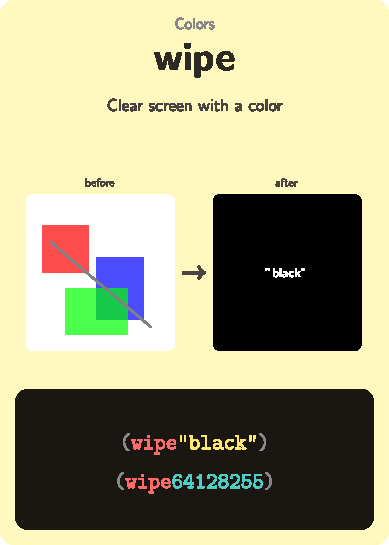
\includegraphics[height=4.5cm]{card-wipe.pdf}%
\hfill%
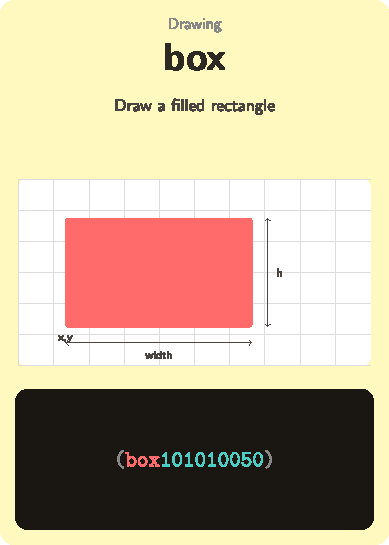
\includegraphics[height=4.5cm]{card-box.pdf}
\caption{Tarjetas de referencia para \texttt{wipe} (limpiar pantalla con color) y \texttt{box} (dibujar rectángulo). Cada tarjeta muestra la firma de la función, un ejemplo visual en una cuadrícula y el código fuente correspondiente.}
\label{fig:cards2}
\end{figure}

\subsection{Imágenes de vista previa social}

El oven genera imágenes de vista previa Open Graph para compartir en redes sociales en URLs estables (p.~ej., \texttt{/kidlisp-og.png}). Los rastreadores de iOS requieren servicio directo de imágenes---no seguirán redirecciones 301 en URLs \texttt{og:image}---por lo que el oven almacena en caché PNGs generados y los sirve con respuestas 200 inmediatas, activando regeneración asíncrona en fallos de caché.

\subsection{Entrega de activos}

Todos los activos de medios se sirven vía DigitalOcean Spaces CDN (\texttt{art-aesthetic-computer.sfo3.cdn.\allowbreak digitaloceanspaces.com}). Las cintas grabadas usan un bucket separado (\texttt{at-blobs-aesthetic-computer}) con un dominio CDN personalizado opcional. Netlify redirige las rutas \texttt{/preview/*} e \texttt{/icon/*} al oven para resolución transparente de URLs.

% ============ 6. IDE ============

\section{Entorno de desarrollo}

El IDE de \kidlisp{} en \texttt{kidlisp.com} proporciona un editor basado en Monaco con resaltado de sintaxis personalizado, un iframe de vista previa en vivo ejecutando el entorno de ejecución de Aesthetic Computer, un panel de consola y controles de reproducción (reproducir/pausar/detener).

Un ``modo deslizador'' permite arrastrar literales numéricos en el editor para ajustar valores en tiempo real---el cursor se convierte en un deslizador horizontal sobre cualquier número, y la vista previa se actualiza continuamente durante el arrastre.

El IDE soporta dos modos de diseño: \emph{studio} (editor de panel dividido, vista previa y consola) y \emph{stage} (editor superpuesto directamente sobre el lienzo a pantalla completa con fondo transparente, todo el chrome oculto). El modo stage está diseñado para contextos de actuación en vivo donde el código mismo se convierte en parte de la salida visual.

% ============ 7. HISTORIA DEL DESARROLLO ============

\section{Historia del desarrollo}
\label{sec:history}

La siguiente línea temporal se reconstruye a partir del historial git del repositorio de Aesthetic Computer (626 commits que tocan \texttt{kidlisp.mjs} entre abril de 2024 y marzo de 2026).

\subsection{Fase 1: Prototipo (abril--junio 2024)}

El desarrollo comenzó el 17 de abril de 2024 con un commit titulado ``mock lisp.'' En tres días, el analizador de S-expresiones estaba funcionando, \texttt{ink} y \texttt{line} aceptaban parámetros numéricos, y los programas podían ingresarse directamente en el prompt de AC. A finales de abril, se añadió \texttt{def} para definiciones de variables. Mayo y junio de 2024 vieron 66 commits añadiendo funciones de dibujo centrales, el constructo de temporización \texttt{later}, \texttt{once} para ejecución única, y publicación anónima de programas. El evaluador alcanzó aproximadamente 1.000 líneas.

\subsection{Fase 2: Pausa (julio 2024--mayo 2025)}

Ningún commit tocó \texttt{kidlisp.mjs} durante 11 meses. El lenguaje existía como un prototipo funcional incrustado en el prompt de AC pero carecía de un backend de almacenamiento, incrustación, audio o un editor dedicado.

\subsection{Fase 3: Expansión rápida (junio--agosto 2025)}

El desarrollo se reanudó en junio de 2025 con 82 commits ese mes. El evaluador creció de 1.760 a 4.965 líneas para agosto. Adiciones clave:

\begin{itemize}
  \item \textbf{Junio 2025}: Analizador de melodías, sintaxis de reloj, modelo de renderizado por fotograma, suite de pruebas (\texttt{kidlisp-spec.js}).
  \item \textbf{Julio 2025}: Backend de almacenamiento MongoDB (\texttt{store-kidlisp.mjs}), generación de códigos cortos, compartición por QR, grabación en cinta y exportación GIF, entrada de micrófono (\texttt{mic}) con animaciones de respaldo.
  \item \textbf{Agosto 2025}: Capas incrustadas (sintaxis \texttt{\$code}) con composición alfa y almacenamiento fuera de pantalla, integración blockchain Tezos para acuñar programas como NFTs, gradientes \texttt{fade}, y optimizaciones de búfer de píxeles.
\end{itemize}

El evaluador superó las 10.000 líneas a finales de septiembre de 2025.

\subsection{Fase 4: Integración de plataforma (septiembre--diciembre 2025)}

Con 108 commits solo en octubre (el mes pico), esta fase integró \kidlisp{} en el ecosistema más amplio de Aesthetic Computer:

\begin{itemize}
  \item \textbf{Septiembre 2025}: Arquitectura de capa 0 (modo borrado), capas de cocción para exportación MP4, correcciones críticas de rendimiento de capas incrustadas.
  \item \textbf{Octubre 2025}: Federación ATProto/Bluesky (programas sindicados como publicaciones en redes sociales), modo PACK para empaquetado independiente de plataforma, modo deslizador para ajuste de parámetros numéricos en tiempo real.
  \item \textbf{Noviembre 2025}: Lanzamiento del IDE \texttt{kidlisp.com} (editor Monaco, vista previa en vivo, consola, controles de reproducción), sistema de traza de ejecución para depuración, flujo de trabajo NFT renombrado de ``OBJKT'' a ``keep.''
  \item \textbf{Diciembre 2025}: Tarjetas de referencia (ilustraciones SVG para cada función), generación de miniaturas IPFS para NFTs, generación de imágenes OG del oven para compartición social, escalado automático de densidad de rendimiento.
\end{itemize}

\subsection{Fase 5: Refinamiento (enero--marzo 2026)}

El evaluador se estabilizó en 15.161 líneas. Las adiciones incluyeron modo caos (febrero 2026), primitivas 3D (\texttt{cube}, \texttt{form}, \texttt{trans}), variables de bandas de frecuencia de audio, el comando \texttt{flip} y modo stage para actuaciones en vivo. El desarrollo cambió de adición de funciones a robustez: corrigiendo regresiones de rendimiento de capas incrustadas, previniendo clasificación errónea del modo caos y mejorando la invalidación de caché.

\begin{table}[h]
\small
\centering
\begin{tabular}{lrl}
\toprule
\textbf{Fecha} & \textbf{Líneas} & \textbf{Hito} \\
\midrule
Abr 2024 & 0 & Commit inicial (``mock lisp'') \\
Jun 2024 & $\sim$1{,}000 & Dibujo, temporización, variables \\
Jun 2025 & 1{,}760 & Se reanuda el desarrollo \\
Ago 2025 & 4{,}965 & Incrustación, audio, almacenamiento \\
Sep 2025 & 10{,}382 & Arquitectura de capas, cocción \\
Dic 2025 & 13{,}877 & IDE, tarjetas, imágenes OG \\
Feb 2026 & 15{,}161 & Modo caos, 3D, refinamiento \\
\bottomrule
\end{tabular}
\caption{Crecimiento del evaluador por conteo de líneas (\texttt{kidlisp.mjs}).}
\label{tab:growth}
\end{table}

% ============ 8. EVALUACIÓN ============

\section{Evaluación}
\label{sec:evaluation}

Las métricas de adopción a marzo de 2026 se muestran en la Tabla~\ref{tab:adoption}.

\begin{table}[h]
\small
\centering
\begin{tabular}{lr}
\toprule
\textbf{Métrica} & \textbf{Valor} \\
\midrule
Total de programas creados & 16.174 \\
Autores únicos & 59 \\
Programas por autor (mediana) & 12 \\
Programas por autor (cuartil superior) & 180+ \\
Profundidad de incrustación (máx. observada) & 7 capas \\
Usuarios registrados de la plataforma & 2.798 \\
\bottomrule
\end{tabular}
\caption{Métricas de adopción (marzo 2026).}
\label{tab:adoption}
\end{table}

\subsection{Analíticas de uso de funciones}

El endpoint de API \texttt{?stats=functions} proporciona conteos de uso de funciones ponderados a través del corpus. Escanea hasta 5.000 programas (ordenados por hits), analiza cada código fuente para extraer llamadas a funciones y devuelve conteos ponderados por popularidad del programa. Esto permite el análisis cuantitativo de qué primitivas gravitan los usuarios. Las funciones más usadas son \texttt{wipe}, \texttt{ink}, \texttt{repeat} y \texttt{circle}---confirmando que los usuarios se involucran principalmente con el dibujo y la iteración.

\subsection{Observaciones}

\textbf{Composición sobre abstracción.} Los usuarios incrustan en lugar de abstraer. Los programas más referenciados son primitivas visuales simples (gradientes, formas, patrones) que sirven como bloques de construcción.

\textbf{Exploración sobre ingeniería.} Los programas son típicamente cortos (menos de 10 líneas). Los usuarios iteran guardando nuevos programas en lugar de editar los existentes, creando caminos de exploración divergentes visibles en las marcas de tiempo de almacenamiento.

\textbf{Aprendizaje social.} Los autores más prolíficos comenzaron viendo y remezclando programas existentes. El sistema de códigos cortos hace que el descubrimiento sea accidental---los usuarios encuentran programas al probar códigos aleatorios.

\subsection{Limitaciones}

\kidlisp{} no es adecuado para programación de propósito general, simulaciones complejas o aplicaciones que requieren persistencia de estado entre sesiones. La falta de funciones definidas por el usuario limita la complejidad de los programas---una elección deliberada, pero una que algunos usuarios avanzados encuentran frustrante.

% ============ 8. TRABAJO RELACIONADO ============

\section{Trabajo relacionado}

\textbf{Programación creativa.} Processing~\citep{reas2007processing} y p5.js~\citep{mccarthy2015p5js} son las herramientas dominantes. OpenFrameworks usa C++. Todas requieren gestionar una estructura de proyecto y entender un lenguaje de propósito general.

\textbf{Programación en vivo.} Hydra~\citep{hydra2019} proporciona programación visual en vivo basada en navegador con encadenamiento de métodos JavaScript pero sin almacenamiento persistente ni funciones sociales. Sonic Pi~\citep{aaron2016sonic} se orienta a la educación musical. Fluxus~\citep{fluxus2007} usó Scheme para visuales 3D pero ya no se mantiene.

\textbf{Lenguajes educativos.} Scratch~\citep{resnick2009scratch} demostró que el compartir social impulsa el engagement en la programación educativa. \kidlisp{} hereda esta idea pero usa sintaxis Lisp basada en texto y se orienta al arte generativo en lugar de la educación general.

\textbf{Lisp para arte.} La biblioteca \texttt{2htdp/image} de Racket~\citep{racket2018} proporciona construcción funcional de imágenes para educación en CS pero se orienta a imágenes estáticas y pedagogía, no a animación en tiempo real con distribución social.

% ============ 9. CONCLUSIÓN ============

\section{Conclusión}

\kidlisp{} demuestra que un lenguaje de dominio específico mínimo---nativo del navegador, sin abstracciones definidas por el usuario, respaldado por una base de datos direccionada por contenido con distribución social---puede soportar una comunidad productiva de practicantes de arte generativo. La idea de diseño clave es que la distribución social (códigos cortos, compartición por URL, incrustación) no es un complemento sino una característica central del lenguaje que moldea cómo los usuarios aprenden, crean y construyen sobre el trabajo de los demás.

El grafo de incrustación, la API de analíticas de uso de funciones y el corpus de más de 16.000 programas con marca de tiempo y atribución de autor constituyen un conjunto de datos para estudiar prácticas de programación creativa, creatividad computacional y cómo los usuarios no expertos aprenden programación funcional a través de la participación social.

\kidlisp{} es código abierto bajo la licencia ISC. El evaluador, la documentación y las herramientas están disponibles en \url{https://github.com/digitpain/aesthetic.computer}. Los programas pueden explorarse y crearse en \url{https://kidlisp.com}.

\vspace{0.5em}
\noindent\textit{Traducido del inglés. Versión original disponible en \url{https://papers.aesthetic.computer}}

\vspace{0.5em}
\noindent\textbf{ORCID:} \href{https://orcid.org/0009-0007-4460-4913}{0009-0007-4460-4913}

% ============ REFERENCES ============

\bibliographystyle{plainnat}
\bibliography{references}

\end{document}
